\documentclass{beamer}
\usetheme{Madrid} % My favorite!
\usepackage{color}
\usepackage{hyperref}
\usecolortheme{orchid} % Simple and clean template
\setbeamercovered{invisible}
\setbeamertemplate{navigation symbols}{} 
\usepackage{natbib}
\usepackage{graphicx}
\usepackage{wrapfig}
\usepackage{soul}
\usepackage{amsfonts}
\usepackage{subfigure}

%
\title[Improving meIRL-based motion modelling]{Improving meIRL-based motion modelling in video
games using general behaviour classification}
\author[Inge Becht]{\large{Inge Becht}\\{\small Supervised by: Sander Bakkes}}
\institute[Universiteit van Amsterdam]
{\large Universiteit van Amsterdam}

\date{\today}
% \today will show current date. 
% Alternatively, you can specify a date.
%
\begin{document}

\begin{frame}
    \titlepage
\end{frame}

\begin{frame}
    \frametitle{Introduction}
    \begin{block}{Problem statement}
        To what extent can general \st{player} \textbf{behaviour} classification improve meIRL-based motion modelling
        in video-games?
    \end{block}
    \begin{itemize}
        \item AI able to anticipate opponent's position
        \item A more human-like AI
        \item Tested on game of Capture the Flag
        \item Adding to existing AI (Terminator)
        \item Capture the Flag
   \end{itemize}
\end{frame}

\begin{frame}
    \frametitle{Motion Models}
    \begin{itemize}
        \item One model for every behaviour, 6 total
        \item learned using maximum entropy IRL(meIRL)
            \begin{itemize}
                \item Deducing reward for actions from agent
                \item Minimizes information loss, more human-like
                    behaviour\citep{6374144}
            \end{itemize}
        \item Features for every tile on grid:
            \begin{itemize}
                \item Shortest distance to flag spawns
                \item Shortest distance to bot spawns
                \item Shortest distance to flag score
                \item Visibility 
            \end{itemize}
        \item Returns probability field
        \item All works, but computation takes time...
    \end{itemize}
\end{frame}
\begin{frame}
\begin{figure}
\centering
\mbox{\subfigure{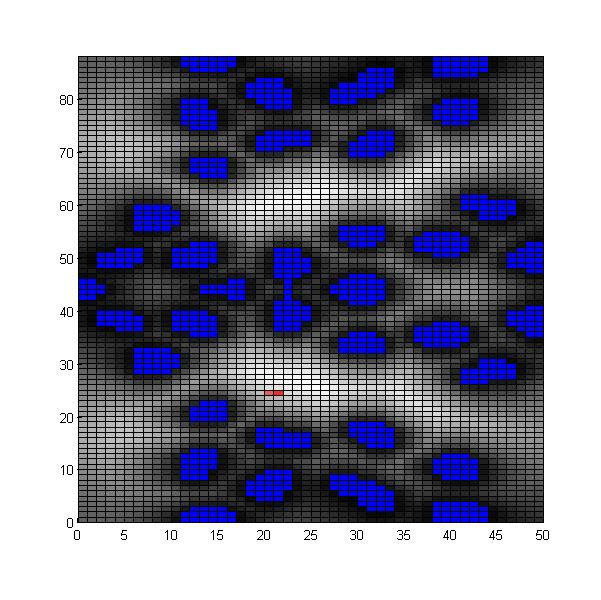
\includegraphics[width=2.3in]{image1.jpeg}}\quad
\subfigure{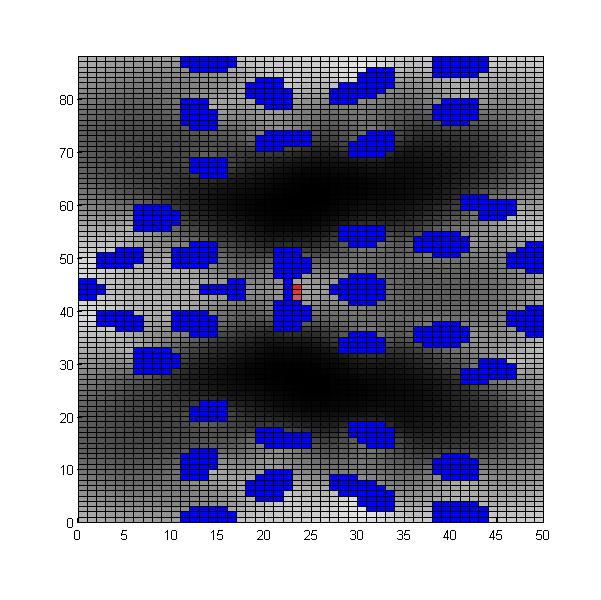
\includegraphics[width=2.3in]{image2.jpeg} }}
\caption{Two example motion models} 
\end{figure}
\end{frame}

\begin{frame}
    \frametitle{Behaviour Classification}
    \begin{itemize}
        \item Acquired Behaviour data consists of Terminator's own behaviour  data
            \begin{itemize}
                \item \emph{What would I be doing if I were in the opponent's
                    situation?}
            \item Assumes the goal is the same for all players.
            \end{itemize}
        \item Features extracted (each \emph{game cycle}):
            \begin{itemize}
                \item bot orientation
                \item position expressed in POI distances
                \item game state
                \item distance to opponent
                \item sees opponent
            \end{itemize}
    \end{itemize}
    \end{frame}

\begin{frame}
    \frametitle{Behaviour Classification Continued}
    \begin{itemize}
        \item Approx. 4200 instances of 6 classes 
        \item  Random Forest Classifier
            \begin{itemize}
            \item 79 \% correct when only using 2 classes (using
                cross validation)
            \item 72 \% correct when classifying all classes (using
                cross validation)
        \end{itemize}
        \item Cons
        \begin{itemize}
        \item Disregards sequential nature of data
        \item Limited performance
        \end{itemize}
        \item Pros
        \begin{itemize}
            \item Fast enough for online classification
            \item Returns Probability of classification
        \end{itemize}
    \end{itemize}
\end{frame}

\begin{frame}
    \frametitle{What's Next?}

    \begin{center}
        \begin{tabular}{| l | l | }
            \hline
            Part & Status \\    \hline
            Creating a working Classifier & \checkmark \\ \hline
            Creating Motion Models using meIRL &  \checkmark \\ \hline
            Using Discrete Propability Propagation & Todo \\ \hline
            Updating histograms & Todo\\
            \hline
        \end{tabular}
    \end{center}
    %\begin{itemize}
    %    \item Putting it all together
    %        \begin{itemize}
    %        \item Add classifier to AI
    %        \item Add Particle Filter to AI
    %        \item Update histograms of  AI
    %        \item Uncertain classifcation? Look at prior classification of
    %            the bot
    %        \end{itemize}
    %    \item Evaluating the research
    %        \begin{itemize}
    %            \item[\checkmark] classification evaluation
    %            \item Examine the errors the motion model makes
    %            \item Mini-competition to test the improvement in performance
    %        \end{itemize}
    %\end{itemize}
\end{frame}

\begin{frame}
    \frametitle{What's Next?}
    \begin{itemize}
        \item Evaluation of research
            \begin{itemize}
                \item[\checkmark] Classification Evaluation
                \item Mini-competition to test the improvement in performance
                    \begin{center}
                        \begin{tabular}{| l | l | }
                            \hline
                        \multicolumn{2}{ |c| }{vs} \\
                            \hline
                            Terminator & Terminator \\ \hline
                            Terminator & Terminator meIRL \\ \hline
                            Terminator & Terminator meIRL w. Classification \\ \hline
                            Terminator meIRL & Terminator meIRL w.
                            Classification\\
                            \hline
                        \end{tabular}
                    \end{center}
                \item Look at general improved trends between old and new meIRL
            \end{itemize}
    \end{itemize}
\end{frame}

\bibliographystyle{apalike}
\begin{frame}
    \frametitle{References}
\bibliography{references}
\end{frame}

\end{document} 
